\documentclass[12pt]{article}
\usepackage{graphicx,float,amsmath,amssymb,url}

\makeatletter
\def\ps@pprintTitle{%
 \let\@oddhead\@empty
 \let\@evenhead\@empty
 \def\@oddfoot{\centerline{\thepage}}%
 \let\@evenfoot\@oddfoot}
\makeatother

\DeclareMathOperator*{\argmax}{arg\,max}

\setlength{\parskip}{1em}
\setlength{\parindent}{0em}

\graphicspath{ {../../static/img/}}

\usepackage[backend=biber]{biblatex}
\bibliography{report}

\begin{document}

\section{Introduction}

% The World's Hardest Game~\cite{game} (TWHG) is a widely-available online Flash game known for its infuriatingly difficult gameplay. In the game, a player selects a move from a discrete set (up, down, left, right, stay) to make at each time step, with the goal of navigating through a series of levels. While the game is deterministic (modulo some random initialization of the enemies), it is a very difficult task for humans to complete, requiring precision, patience, and often a difficult-to-discover strategy for movement. However, the set of actions to be taken at any given time step is bounded in size, and the reward for an action is easily calculated. Thus, the game is a good candidate for a reinforcement learning-based model.

The World's Hardest Game~\cite{game} (TWHG) is a widely-available online Flash game known for its infuriatingly difficult gameplay. In the game, a player selects a move from a discrete set (up, down, left, right, stay) to make at each time step, with the goal of navigating through a series of levels. In order to complete a level, the player must collect all on-screen coins, avoid collision with any enemies, and reach the area designated as the end zone. While the game is deterministic (modulo some random initialization of the enemies), it is a very difficult task for humans to complete, requiring precision, patience, and often a difficult-to-discover strategy for movement. However, the set of actions to be taken at any given time step is finite, and the reward for an action is easily calculated. Thus, the game is a good candidate for a reinforcement learning-based model.

\begin{figure}[H]
  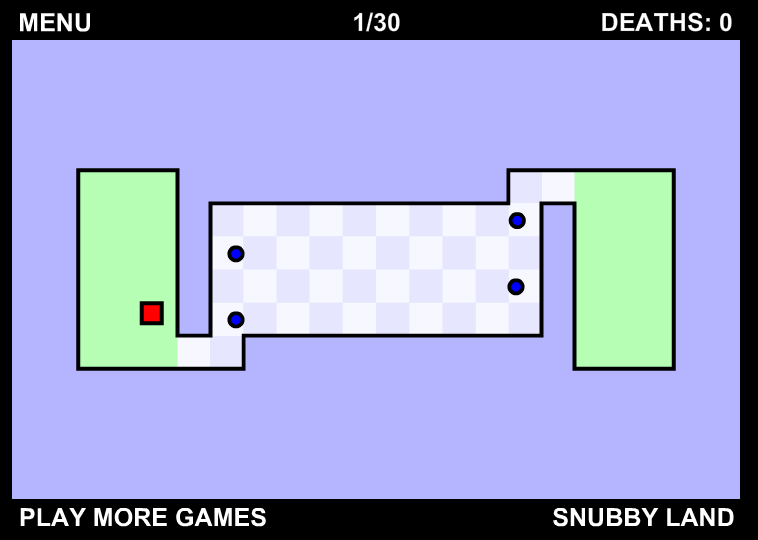
\includegraphics[width=1\textwidth]{report/hardest_game}
  \centering
  \caption{Level 1 of TWHG}
  \label{fig:twhg}
\end{figure}

Deep learning, combined with classic reinforcement learning techniques, allows one to learn a action-selection policy on complicated, long games that have significant delays between action and reward. Furthermore, a CNN is capable of taking pixel inputs from frames of a game simulator and learning a representation of the game state from them. Thus, it is theoretically possible to have a game-winning strategy learned simply by ``playing'' a game over and over, and observing the results.

The original goal of this paper was to use the Deep Q-learning with Experience Replay technique pioneered by DeepMind~\cite{deepmind} to train a model that was capable of beating TWHG, surpassing the performance of even the most skilled human player. After weeks of training, it became clear that acheiving this is beyond the scope of the paper, with the best models barely managing to navigate the player out of the starting area. Therefore, we instead explored several related ``toy'' games (all with a similar premise), testing the techniques and hyperparameters laid out in the DeepMind paper against two baselines: a random model, and a $\epsilon$-greedy model.

We tested my architechture and model against increasingly complicated toy games, attempting learning both with pixel inputs as well as by directly feeding in a representative state vector. The results show that training with image inputs takes prohibitively long, where as directly feeding in state vectors results in a model that outperforms both the baselines within days. Furthermore, the learned models take actions that are intuitive to a human player, with no seeding required.

All the referenced implementation code for this paper can be found online at \url{https://github.com/yasyf/hardest-game}.

\section{Background}

\subsection{Reinforcement Learning}

Q-learning, in which an agent optimizes a game-specific \textit{reward function} by taking an \textit{action} which maximizes the discounted sum of future rewards (\textit{Q values}), is a popular reinforcement learning technique for interacting with an \textit{environment} and set of actions that can be modelled as a finite Markov decision process (MDP). The solution can be discovered via a simple value-iteration update algorithm~\cite{Watkins1992}.

At its heart, the process works as follows. At each time step, the actor selects an action from $\mathcal{A}$, the space of actions available in the given environment $\varepsilon$. This action is passed to a simulator (implemented in our case for each game learned), which modifies $\varepsilon$, without revealing its internal state. The agent then observes state vector representing the $\varepsilon$, as well as a reward $r_t \in \mathbb{R}$. This sequence of actions, observations, and rewards is then used to solve the MDP they represent. Future rewards are discounted by a rate $\gamma$.

\subsection{Deep Reinforcement Learning}

Advances in deep learning have brought about the advent of Deep Q-learning, which relies on the same underlying principles as Q-learning, but replaces the central lookup table with a neural net, allowing one to learn a function apprimator to the $Q$ function in a much larger and sparser action space, without exploring every possible set of moves (which can often be intractable for more complicated games). Furthermore, convolutional layers of the net allow the model to learn directly from game frames (or in our case, several stacked frames), decreasing the amount of structured information that needs to be supplied.

Gradient descent technques were used to optimize the parameters of the network. The architechture was a CNN which took $84 \times 84 \times 4$ vectors, and contained two hidden layers: 16 $8 \times 8$ filters of stride $4$ and 32 $4 \times 4$ filters of stride $2$. This was followed by a 256-node fully-connected hidden layer of ReLU, and an output layer with $|\mathcal{A}|$ linear nodes. This will become the starting point of the models described in this paper.

\subsection{Simulators}

As a Flash-based game, TWHG is easy to simulate. Using headless browser wrappers such as Selenium, it is possible to launch instances of Google Chrome and load the SWF containing the game's code without user intervention. Simulating user moves and extracting state is done through the bare-bones JavaScript API exposed by the Flash runtime~\cite{flashjs}. Internal state can be read using the \texttt{TGetProperty} and \texttt{GetVariable} methods, and written using the corresponding \texttt{Set*} methods. Part of the contribution of this paper is a generic Python-based simulator~\cite{simulator} which can interact with Flash-based games and report observable state, as well as capture frames for later processing.

\subsection{Games}

Techniques similar to the above (albeit with a fully-fleged console emulator) were successfully used to play Atari 2600 games at an expert level by the DeepMind team~\cite{deepmind} in 2013. Previously, attempts were made by Brodman and Voldstad~\cite{Brodman2012QwopL} to play games like QWOP~\cite{qwop} by modelling the game in detail, and extracting precise state vectors, with classic RL techniques. Another recent application of RL (though not Deep RL) to games is the use of Q-learning to play Super Mario with a 90\% win rate\cite{Liao2012Cs229FR}. We could not find any published examples of using Deep Q-learning on a simulated Flash game, though recently-launched platforms like the OpenAI Universe (\url{https://universe.openai.com}) open the gateway for many similar attempts.

\section{Methods}

\subsection{Games}

In addition to TWHG, described above, we implemented several simple games of varying difficulty, in order to test the efficacy of the techniques and models presented in this paper within a limited span of time.

\subsubsection{TG1D}

The first game (TG1D) is a very simple game, involving a 1-dimensional 4-square grid that has one enemy randomly placed on one of the middle two squares. The enemy $e$ appears and dissapears with a random phase, and the goal of the player $p$ is to move from the first square to the last, without ever being in the same square as the in-phase enemy. The possible moves for the player are $\{\texttt{left}, \texttt{right}, \texttt{stay}\}$. The observable state vector $S$ for this game is as follows.

\[S_{x} =
\begin{cases}
  -2 & \text{if } e = x \text{ and } p = x \\
  -1 & \text{if } e = x \\
  1 & \text{if }  p = x \\
  0 & \text{else} \\
\end{cases}
\]

\subsubsection{TG2D}

TG2D is the natural 2-dimensional progression of this simple game. The game is played on a $4 \times 4$ grid, with the starting location for $p$ at $(0, 0)$ and the goal location at $(3, 3)$. A single enemy occupies a random square selected from those that are not the start or goal, with a random phase. The objective is the same.  The possible moves for the player are $\{\texttt{left}, \texttt{right}, \texttt{down}, \texttt{up}, \texttt{stay}\}$. $S$ for this game follows as expected from the 1-dimensional case, though it is now a matrix (which is flattened to produce the final state vector).

\subsubsection{TG2D-H}

TG2D-H is the exact same game as TG2D, but with multiple enemies. Each enemy is sampled from the squares remaining after removing the start, goal, and any square that currently has an enemy assigned to it.

\subsection{Learning}

To implement the neural net architechture for this model, we used the popular TensorFlow library. Simple abstractions were build around 2D-convolutional and fully-connected layers, which were strung together to test various architechtures. At times, reference was made to various existing implementation of Deep Q-learning in TensorFlow \cite{deep-rl-tensorflow} \cite{dqn-tensorflow}.

The output of the net represented the Q-estimate for each action, with the best action defined as $\argmax_{a \in \mathcal{A}} Q(t, a)$. The loss function used for optimization is the mean-squared-error of the Q-estimate predicted for a given action $a$ at time $t$, and the ``realized'' Q-value, which is the known reward for $a$ at $t$ added to the discounted Q-estimate of the best action at the state $t+1$, given $a$ was made at $t$. Below we give the formula for the loss of a minibatch $\mathcal{B}$, sampled from the replay memory $\mathcal{M}$.

\[\ell = \frac{1}{|\mathcal{B}|} \sum_{t \in \mathcal{B}} \left[\texttt{clip}\left(Q\left(t, a_t\right) - \left[r_{t,a}  + \gamma \max_{a \in \mathcal{A}} Q\left(t+1, a\right)\right]\right)\right]^2\]

The difference in Q-estimate for $t$ and ``realized'' Q-value is clipped to be in the range $[\delta_{-}, \delta_{+}]$, as reccomended by the DeepMind paper, in order to limit the scale of the error gradient. Several values where tried for the bounds of this range. Finally, the Adam optimizer was used to optimize this loss function given the game samples.

Samples were provided using the Experience Replay technique described in the DeepMind paper, with an $\epsilon$-greedy policy for selecting optimal moves (with $\epsilon$ controlling how often random moves were made, in order to force exploration, as opposed to the move suggested by the current Q-estimates). The replay memory of each episode (from which minibatch training points are sampled) is first seeded by filling the history $\mathcal{H}$ (which holds the stacked inputs to the model for the given timestep) with $|\mathcal{H}|$ frames of the player making the \texttt{stay} move. This has the nice property of exposing the model to the motion patterns of enemies, which aids in predicting where enemies will appear when the player starts moving.

\begin{figure}[H]
  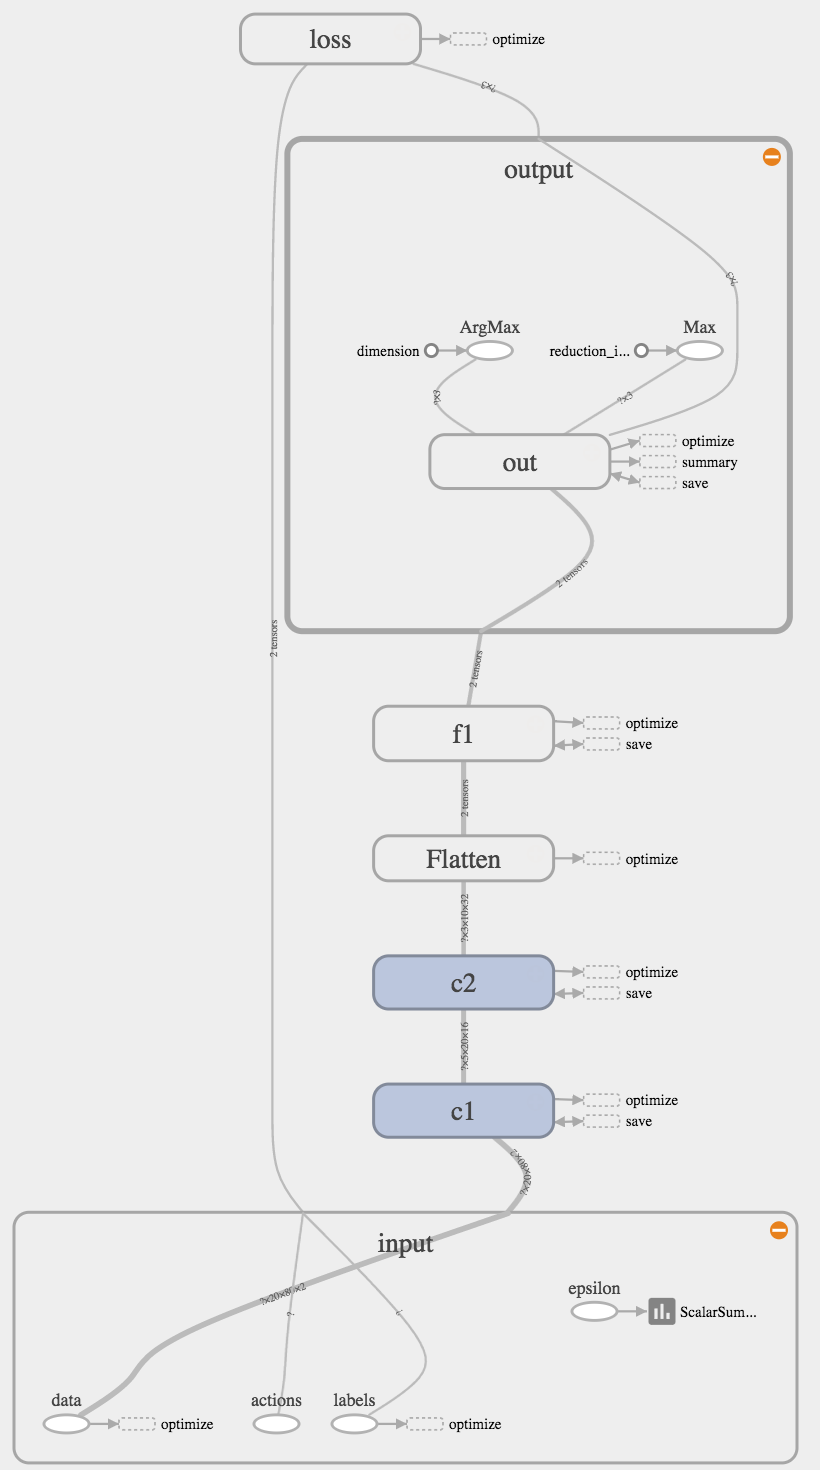
\includegraphics[height=1\textwidth]{report/image_graph}
  \centering
  \caption{TensorFlow Graph of Net Architechture With Images}
  \label{fig:imgraph}
\end{figure}

When feeding in frame images, the architechture used was exactly as described in the DeepMind paper~\cite{deepmind} (CNN), with either 3 or 5 output nodes, depending on the game. When feeding in state vectors, we instead use 2 fully-connected (FC) hidden layers, one with 128 and one with 64 ReLU nodes. Some alterate architechtures were experimented with; further work could include testing out more, particularly in the non-image case. Figure \label{fig:trainingwinrate} shows the exponentially-weighted moving average of the win rate during training for two archiechtures: $[128, 64]$ (organge) and $[256, 256]$ (purple).

\begin{figure}[H]
  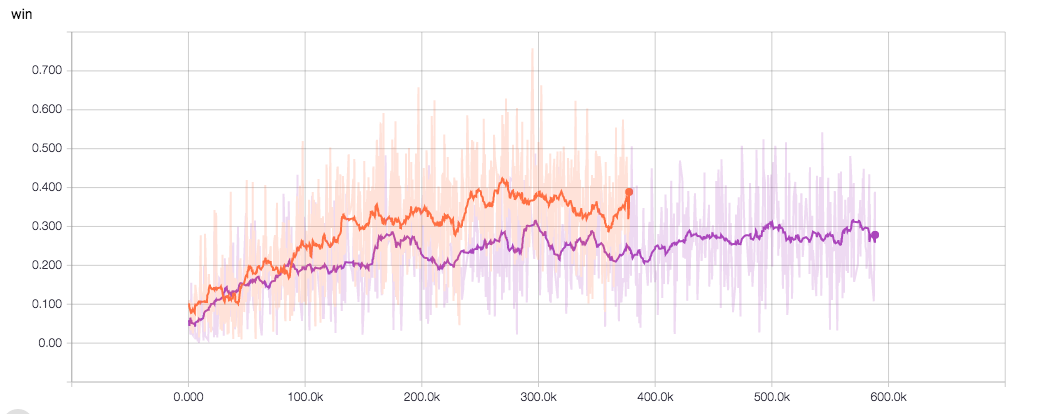
\includegraphics[height=1\textwidth]{report/TG2D-H_training_winrate}
  \centering
  \caption{Training Win Rates of TG2D-H}
  \label{fig:trainingwinrate}
\end{figure}

\subsection{Hyperparameters}

Most of the hyperparameters in the system were copied from the DeepMind paper, then modified and tuned as appropriate for this set of games. Where the value of the hyperparameters

A $\gamma$ value of $0.90$ was used initially, which sufficiently penalizes future rewards in order to discourage the player from getting ``stuck'', which occurs when all non-\texttt{stay} actions have negative Q-values (common near the start of a training session). We experimented increasing this to $0.99$, expecting that increasing the value of future rewards would make the resulting player more risk-averse. Indeed, this was confirmed, with the resulting model often causing the player to \texttt{stay} ad infinitum.

$\epsilon$, the parameter which controls how often a random action is selected when the model is exploring, starts at $0.9$ and is linearly annealed to $0.1$, over a lifetime of $10^5$ frames. This was originally much lower, but was increased to closer match DeepMind's $10^6$, as lower values would allow the model to converge on local solutions that were sub-optimal due to a lack of sufficient exploring. Thus we see that some level of stochastisity is required in order to sufficiently uncover the state space.

A minibatch size of 32 was used. This was sampled from a replay memory size of $10^5$, an order of magnitude less than the DeepMind paper. While $10^6$ was initially used, using a lower value allowed us a discernable increase in training time and performance, with negligible impact on the results.

The difference between predicted and expected Q-values was initially not clipped, resulting in blowup of the error gradient and huge sensitivity to slight changes in the reward function. As a result, we initially clipped the values to be in $[-1, 1]$, as in the DeepMind paper. However, this did not allow for enough variance to accuratley reflect the games at hand, so this was ultimately changed to be $[-10, 10]$.

Determining $|\mathcal{H}|$, the number of stacked images to feed into the CNN, required some experimentation. For the smaller, simpler games, a history size of 2 was optimal. As the games grow more complex, we settle on $|\mathcal{H}| = 3$ (an average loss of $1.36$ vs $2.11$ after 150k frames).

\begin{figure}[H]
  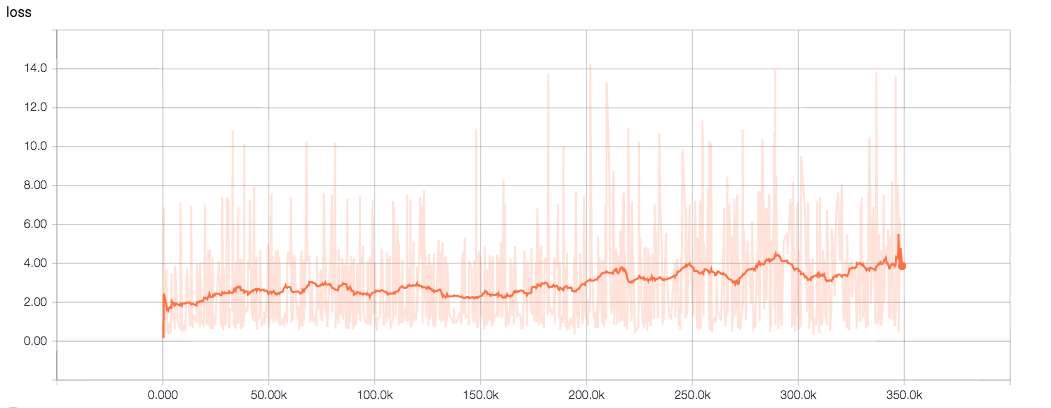
\includegraphics[width=1\textwidth]{report/history_size_3}
  \centering
  \caption{Loss Over Time For TG2D with $|\mathcal{H}| = 3$}
  \label{fig:tg2dh3loss}
\end{figure}

A final decision to be made was whether to feed in pixel matrices directly (thereby using the CNN architechture), or to extract state vectors and use the FC architechture. As is shown in the results, using CNN allows us to encode much less information about the game when learning the model, but has a prohibitively long training period. Thus we ultimately report our best results with state vector inputs.

\section{Results}

Following the tuning of the above hyperparameters, we ran our best models, as well as two baselines, on each of the three toy games. We also attempted to train a model on TWHG. However, the training time was prohibitive, on account of the Flash simulation taking three to four orders of magnitude longer to modify $\varepsilon$ than the simulators we built for the toy games. Thus, after over a week of training, we did not have any significant results to report.

The win rates reported below are averaged over $10$ runs, each containing $1000$ games, for a total of $10000$ samples.

\subsection{Baselines}

\subsubsection{Random}

We implemented a basic random model as a baseline. The model samples an action from a uniform distribution over $\mathcal{A}$.

\begin{figure}[H]
  \begin{tabular}{c | c}
    Game & Win Rate (\%) \\ \hline
    TG1D & 28.85 \\ \hline
    TG2D & 36.95 \\ \hline
    TG2D-H & 9.18 \\
  \end{tabular}
  \centering
\end{figure}

\subsubsection{$\epsilon$-Greedy}

Our next baseline was a $\epsilon$-greedy model that sampled a uniformly random action with probability $\epsilon$, and took the greedy action at $t+1$ based on the rewards at $t$ with probaility $1 - \epsilon$. For the below values, we used $\epsilon = 0.05$.

\begin{figure}[H]
  \begin{tabular}{c | c}
    Game & Win Rate (\%) \\ \hline
    TG1D & 92.06 \\ \hline
    TG2D & 77.76 \\ \hline
    TG2D-H & 47.98 \\
  \end{tabular}
  \centering
\end{figure}

\subsection{Deep Model}

We ran the best model over serveral training runs for each game, and present the results below. For any game more complex than the basic 1-D toy game, we see that our Deep Q-learning model outperforms the naive $\epsilon$-greedy model.

For the simple TG1D, we hypothesize that such a simple game can effectively be mastered with a greedy strategy, and that our function approximator could not match these results given the limited training time.


\begin{figure}[H]
  \begin{tabular}{c | c}
    Game & Win Rate (\%) & \# Training Frames \\ \hline
    TG1D &  \\ \hline
    TG2D & 78.91 & 240k \\ \hline
    TG2D-H &  \\
  \end{tabular}
  \centering
\end{figure}

\section{Discussion}

An interesting note is that the best-performing deep model for TG1D simply learned to always move \texttt{right} unless there is an enemy present, in which case it \texttt{stay}s for one turn, then continues to move right. This is almost the correct (greedy) strategy, but does not take into account the case of enemies which are on screen for more than one turn.

Focusing on the more complicated (toy) games, we can make some revealing observations.

\begin{figure}[H]
  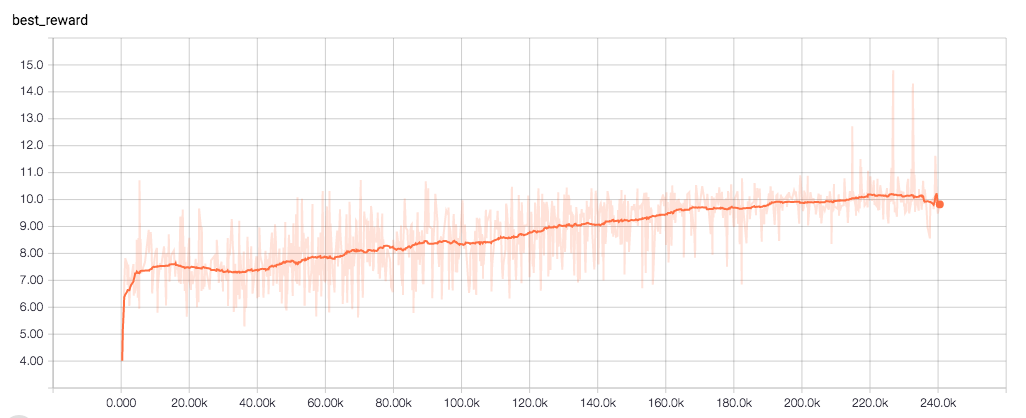
\includegraphics[height=1\textwidth]{report/TG2D_best_reward}
  \centering
  \caption{Max Q-value Estimate Over Time For TG2D}
  \label{fig:maxqv}
\end{figure}

\begin{figure}[H]
  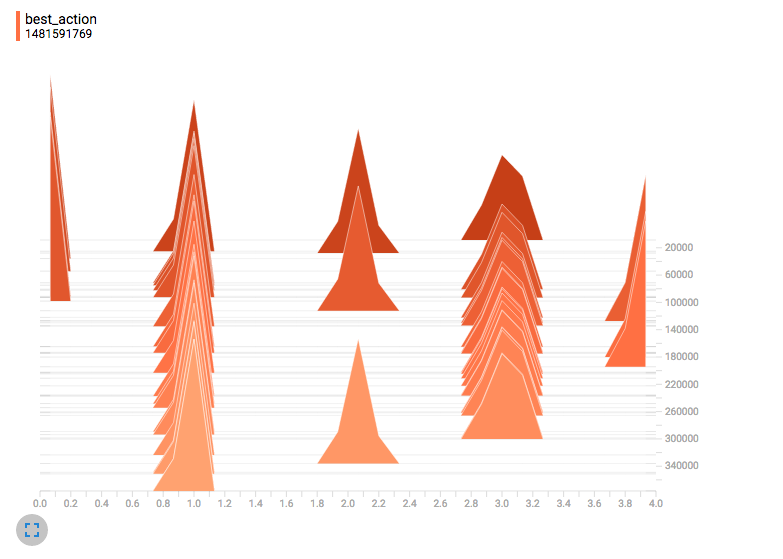
\includegraphics[height=1\textwidth]{report/TG2D-H_best_action_hist}
  \centering
  \caption{Time over Distribution of Best Action for TG2D-H}
  \label{fig:bahist}
\end{figure}

\begin{figure}[H]
  \begin{subfigure}{0.19\textwidth}
    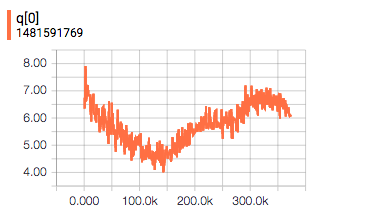
\includegraphics[width=1\textwidth]{report/TG2D-H_action_q/q0}
    \caption*{\texttt{Up}}
    \centering
  \end{subfigure}
  \begin{subfigure}{0.19\textwidth}
    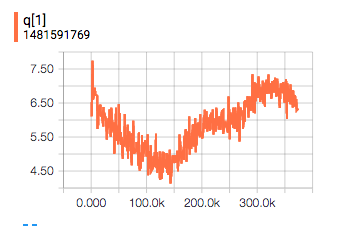
\includegraphics[width=1\textwidth]{report/TG2D-H_action_q/q1}
    \caption*{\texttt{Down}}
    \centering
  \end{subfigure}
  \begin{subfigure}{0.19\textwidth}
    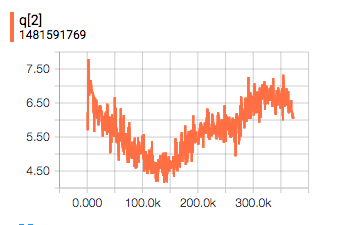
\includegraphics[width=1\textwidth]{report/TG2D-H_action_q/q2}
    \caption*{\texttt{Left}}
    \centering
  \end{subfigure}
  \begin{subfigure}{0.19\textwidth}
    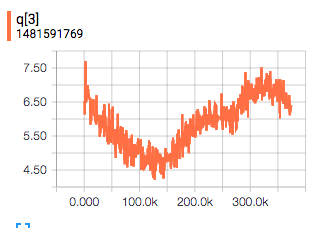
\includegraphics[width=1\textwidth]{report/TG2D-H_action_q/q3}
    \caption*{\texttt{Right}}
    \centering
  \end{subfigure}
  \begin{subfigure}{0.19\textwidth}
    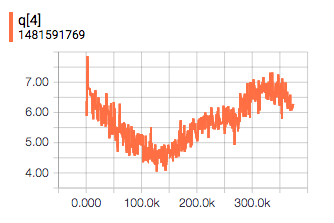
\includegraphics[width=1\textwidth]{report/TG2D-H_action_q/q4}
    \caption*{\texttt{Stay}}
    \centering
  \end{subfigure}
  \centering
  \caption{Per-Action Q-value Estimates Over Time For TG2D-H}
  \label{fig:maxperaqv}
\end{figure}

\subsection{Challenges}

- figuring out flash ``registers''
- training time, particularly with flash simulator, solved with pool of simulators
- balance between reward function being too specific and not allowing for unintuitive exploration, and being conservative enough that player just gets stuck
- initialization

\section{Conclusion}

\subsection{Further Work}

\pagebreak
\printbibliography

\end{document}
